\documentclass[12pt, oneside]{article}
\usepackage{tikz} 
\usepackage{fancyvrb}
\usepackage{soul}
\usepackage{color}
\usepackage{listings}


\definecolor{codegreen}{rgb}{0,0.6,0}
\definecolor{codegray}{rgb}{0.5,0.5,0.5}
\definecolor{codepurple}{rgb}{0.58,0,0.82}
\definecolor{backcolour}{rgb}{0.95,0.95,0.92}

\lstdefinestyle{mystyle}{
    backgroundcolor=\color{backcolour},   
    commentstyle=\color{codegreen},
    keywordstyle=\color{magenta},
    numberstyle=\tiny\color{codegray},
    stringstyle=\color{codepurple},
    basicstyle=\ttfamily\footnotesize,
    breakatwhitespace=false,         
    breaklines=true,                 
    captionpos=b,                    
    keepspaces=true,                 
    numbers=left,                    
    numbersep=5pt,                  
    showspaces=false,                
    showstringspaces=false,
    showtabs=false,                  
    tabsize=2
}

\lstset{style=mystyle}



%%%%%%%%%%%%%%%%%%%%%%%%%%%%
%%   Zusaetzliche Pakete  %%
%%%%%%%%%%%%%%%%%%%%%%%%%%%%
\usepackage[ngerman, english]{babel}
\usepackage{acronym}
\usepackage{enumerate}  
\usepackage{a4wide}
\usepackage{fancyhdr}
\usepackage{graphicx}
\usepackage{palatino}
\usepackage{float}
\usepackage{csquotes}
\usepackage[bookmarks]{hyperref}

\usepackage[style=authoryear-comp,dashed=false,natbib=true,backend=bibtex,maxnames=2]{biblatex}
\usepackage[justification=centering, labelfont=bf, textfont=bf]{caption}
\usepackage[a4paper, margin=0cm, left=3cm, top=2.5cm, right=2cm, bottom=3.5cm]{geometry} 
\usepackage{etoolbox}
\usepackage{acronym}
\usepackage{titlesec}
\usepackage[titles]{tocloft}
\usepackage{fontspec}

\setlength\cftparskip{-2pt}
\setlength\cftbeforesecskip{0pt}
\setlength\cftaftertoctitleskip{0pt}

\setmainfont{Times New Roman}

\DeclareCaptionFormat{myformat}{\fontsize{10}{0}\selectfont#1#2#3}
\captionsetup{format=myformat}

\setlength\parindent{0pt}
\setlength{\parskip}{6pt}
\setlength{\headheight}{0.8cm}

\linespread{1.25}

%\setlength{\cftbeforesecskip}{1.75pt}

\renewcommand{\cftfigpresnum}{Abbildung }
\renewcommand{\cfttabpresnum}{Tabelle }

\renewcommand{\cftfigaftersnum}{:}
\renewcommand{\cfttabaftersnum}{:}

\setlength{\cftfignumwidth}{2.75cm}
\setlength{\cfttabnumwidth}{2cm}

\setlength{\cftfigindent}{0cm}
\setlength{\cfttabindent}{0cm}

\renewcommand{\figurename}{Abbildung}
\renewcommand{\tablename}{Tabelle}


%%%%%%%%%%%%%%%%%%%%%%%%%%%%%%%%%%%%%%%%%%%%%%%%%%%%%
%%  Definition des Deckblattes und der Titelseite  %%
%%%%%%%%%%%%%%%%%%%%%%%%%%%%%%%%%%%%%%%%%%%%%%%%%%%%%

\newcommand{\JMUTitle}[9]{

  \thispagestyle{empty}
  \vspace*{\stretch{1}}
  {\parindent0cm
  \rule{\linewidth}{.7ex}}
  \begin{flushright}
    \vspace*{\stretch{1}}
    \bfseries\Huge
    #1\\
    \vspace*{\stretch{1}}
    \bfseries\large
    #4
  \end{flushright}
  \rule{\linewidth}{.7ex}

  \vspace*{\stretch{1}}
  \begin{center}
    
\includegraphics[width=2in]{GU-Logo-blau-gross} \\
    \vspace*{\stretch{1}}
    \Large #3 \\

    \vspace*{\stretch{2}}
   \large Institute for Computer Science\\
    \large Goethe University Frankfurt\\
    \vspace*{\stretch{1}}
    \large supervised by: \\ #8 \\[1mm]

  \end{center}
}

\newcommand{\Zusammenfassung}[2]{
    \section*{#1}
    \addcontentsline{toc}{section}{#1}%
    \markboth{#1}{#1}
    \noindent
    #2
    \newpage
}


%%%%%%%%%%%%%%%%%%%%%%%%%%%%
%%  Bibtex File einbinden %%
%%%%%%%%%%%%%%%%%%%%%%%%%%%%

\addbibresource{literature.bib}  


%%%%%%%%%%%%%%%%%%%%%%%%%%%%
%%  Beginn des Dokuments  %%
%%%%%%%%%%%%%%%%%%%%%%%%%%%%


\begin{document}

\DeclareRobustCommand{\hlcyan}[1]{{\sethlcolor{cyan}\hl{#1}}}
\DeclareRobustCommand{\hlgreen}[1]{{\sethlcolor{green}\hl{#1}}}
\DeclareRobustCommand{\hlred}[1]{{\sethlcolor{red}\hl{#1}}}



\titlespacing{\section}{0pt}{0pt}{0pt}
\titlespacing{\subsection}{0pt}{6pt}{0pt}
\titlespacing{\subsubsection}{0pt}{6pt}{0pt}

  \JMUTitle
      {Optimizing a Natural Language Processing pipeline for the automatic creation of RDF data}                                % Titel der Arbeit
      {Kurztitel der Arbeit}                            % Muss in die Kopfzeile passen
      {Bachelor Thesis}       % Art der Arbeit
      {Dambowy, Nils }                              % Vor- und Nachname des Autors
      {TT.MM.JJJJ}                                      % Tag der Anemeldung 
      {TT.MM.JJJJ}                                      % Tag der Abgabe
      {Bachelor Informatik}           % Studiengang
      {Dr. Karsten Tolle}
      { }                                                              % Matrikelnummer 
\newpage
\pagenumbering{Roman}
%%%%%%%%%%%%%%%%%%%%%%%%%%%%%%%%%%%%%%%%%%%%%%


%%%%%%%%%%%%%%%%%%%%%%%%%%%%
%%  Inhaltsverzeichnis  %%
%%  wirt automatisch erstellt  %%
%%%%%%%%%%%%%%%%%%%%%%%%%%%%


\tableofcontents


\newpage
\pagenumbering{arabic}
\setcounter{page}{1}
  
  
%%%%%%%%%%%%%%%%%%%%%%%%%%%%
%%  Hauptteil  %%
%%%%%%%%%%%%%%%%%%%%%%%%%%%%

\newpage

\thispagestyle{empty}
\section*{Statement of authorship}
\thispagestyle{empty}
\textbf{In accord to §25 par. 11 of the examination regulations 2011:}\\
I hereby declare that I am the sole author of this bachelor thesis and that I have not used any sources other than those listed in the bibliography and identified as references. I further declare that I have not submitted 
this thesis at any other institution in order to obtain a degree.
\vspace{4\baselineskip}\\
Frankfurt, the \today \hfill Dambowy, Nils
\vspace{4\baselineskip}\\

\newpage
\section*{Abbreviations} \label{abv}
\begin{center}
\begin{tabular}{p{6cm}|p{6cm}}
CN & Corpus Nummorum\\
\hline\\
RDF & Resource Description Framework\\
\hline\\
NLP & Natural Language Processing\\
\hline\\
CN & Corpus Nummorum\\
\hline\\
CN & Corpus Nummorum\\
\hline\\
CN & Corpus Nummorum\\
\hline\\
\end{tabular}
\end{center}
\newpage

%\section{Abstract} \label{abstract}
%This thesis reviews the implementation of a pipeline used for the creation of RDF data from a given database. To optimize the pipeline, the single steps were automatized and the function of external software was replicated. %As a result only the input has to be specified by the user.

\section{Introduction} \label{introduction}
Numismatics is the academic discipline focussing on the study of different forms of currency, including e.g. coins, paper money or medals. These objects can be as old as 200 years BC, modern numismatics usually begins at around 1750. Numismatists made it their task to collect, preserve and categorize these archaeological findings and thereby play an important role in the enlightenment of our history. For example when it comes to determining the date of an archaeological site, coins can be of great use since coinage could indicate a time span or the distance from its place of discovery to its origin could tell us about the mobility during these times. In our current time most numismatic institutions have to go through the challenge of finding an adequate way of managing their data and mostly\footnote{http://nomisma.org/datasets} really on databases. In this thesis I am focussing on the \hyperref[cn]{\textbf{CN}} database, which will be further explained in a later chapter. Currently working with this database is the \textbf{D4N\textsuperscript{4}} (Data quality for Numismatics based on Natural language processing and Neural Networks)\footnote{http://www.bigdata.uni-frankfurt.de/d4n4/} project which goal it is to improve the assignment of existing data(descriptions or images) to different research portals. The assignment is done in two different ways. Firstly the assigning is done with \hyperref[nlp]{\textbf{Natural Language Processing}} which extracts conditions and description and lastly image recognition is used to recognize the coin. Furthermore the project aims to continue the development and implementation of tools useful for numismatic research portals.
\subsection{Problem description} 
In this thesis I am optimizing a currently existing \hyperref[nlp]{\textbf{Natural Language Processing}} pipeline, which will be described in more detail in chapter 5.1. The pipeline consists of two parts. First \hyperref[nlp]{\textbf{Natural Language Processing}} is used to extract a name entities (see \hyperref[ner]{\textbf{Name Entity Relationship}}) and word relationships (see \hyperref[re]{\textbf{Relationship Extraction}}) out of the \hyperref[cn]{\textbf{CN}} database and afterwards written back again. Lastly, with new data and the programm \hyperref[d2r]{\textbf{D2RQ}} \hyperref[rdf]{\textbf{RDF}} data is created with the aim to be published later. Currently the whole process, from the execution of the notebooks to the setup of the D2RQ program has to be done manually. To improve this, the goal of this thesis is to refine the state of current pipeline by automating the process of the NLP and creation of RDF data without having to rely on the tools D2RQ offers. At the end the whole execution of the pipeline should require as little as possible human input. When  given a coin description as an input it should return the results in the RDF format.
\subsection{Thesis strucutre}
In the following chapter I am going go to discuss the CN project and its successor, the D4N4 project which is the database the pipeline is working with. Furthermore in \hyperref[bg]{\textbf{chapter 2}} technical background information about the different technologies used is given to understand the functionality of the new and old pipeline. Afterwards, in chapter 4, the state of current pipeline and the implementation of the revised one is discussed. Both pipelines will also be compared in this chapter. Chapter 5 leaves room for the conclusion and the outlook.
\newpage

\subsection{Related work}
\newpage

\section{Background}\label{bg}
\subsection{Corpus Nummorum} \label{cn}
The Corpus Nummorum \textbf{(CN)} is a  research database, which is  the result of the joint work of the Münzkabinett Berlin, Berlin-Brandenburg Academy of Sciences and Humanities (BBAW) and the Big Data Lab of Goethe University, with the motivation to offer ancient Greek coinage for research purposes.\footnotemark[1]
It contains information about coins with origin in the regions of Lower Moesia, Thrace, Mysia, and the Troad. Added together, the database contains information about approx. 27,500 coins, 14,000 coming from the area of Thrace and 14,500 from the remaining regions. It is also possible to contribute coins to the database yourself.

\begin{figure}[!htb]%
    \centering%
    \begin{minipage}{.5\textwidth}%
        \centering%
        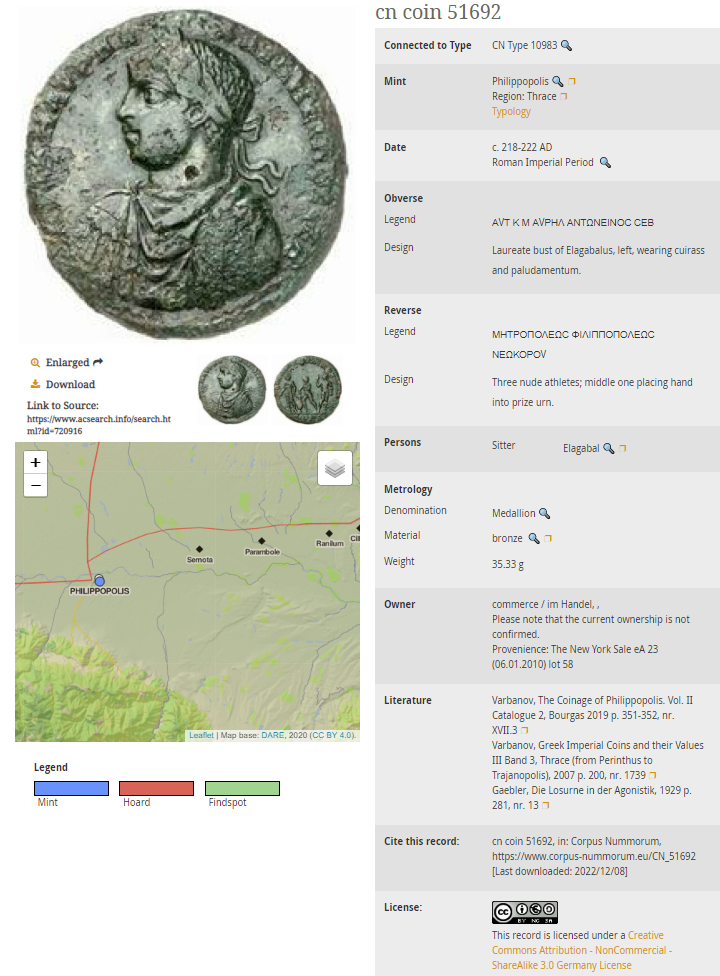
\includegraphics[scale=0.4]{coin_example.png}\\
        \textbf{An example of a coin in the database}\footnotemark[2]%
        \label{fig:coin_example}%
    \end{minipage}%
    \begin{minipage}{0.5\textwidth}%
       All of this information is accessible through the  CN Online Website by using the provided search tool, which lets you filter coins by e.g. epoch, tribe, weight or material. Beside the mentioned characteristics, the CN offers text descriptions of the depicted images on the front- and back side of the coins. To allow a better comparison between different coins, all properties have to be entered in accord to a standardized scheme.\footnotemark[3]  This not only guarantees the previous mentioned upsides but also make entering coins more accessible since e.g. volunteers do not have to worry about having to come up with a scheme themselves. The scheme offers guidelines on how to describe the obverse and reverse of the coin, figures or architecture, portraits, scenes or some general information on how properly describe a coin.
       After a submitting a coin, it has to reviewed before it is published.
    \end{minipage}%
    
\end{figure}%
\footnotetext[1]{https://www.corpus-nummorum.eu/about}
\footnotetext[2]{https://www.corpus-nummorum.eu/coins/51692}
\footnotetext[3]{https://www.corpus-nummorum.eu/pdf/ExternalCoinEntry.pdf}
\newpage
\subsection{D4N4}
The \textbf{D4N\textsuperscript{4}} is research project and a successor of the \textbf{Corpus Nummorum} project. The Name of the project is abbreviated from "Data quality for Numismatics based on Natural language processing and Neural Networks". The project aims to improve the usage of the many available images and descriptions of coins by classifying and assigning them to the different databases. Officially starting in the July of 2021, the project, much like its predecessor is the collaborative effort of the Münzkabinett Berlin, Berlin-Brandenburg Academy of Sciences and Humanities (BBAW) and the Big Data Lab of Goethe University. It achieves that by continuing and driving the development of tools forward which are needed for numismatics.
\subsection{Natural Language Processing} \label{nlp}
NLP deals with the processing of \textit{natural} Language. The term natural referring to the creation of the language which was natural e.g. from through human conversation unlike artificially created languages like programming languages. The language is given as input in text form for analyzation.
Two different forms are being used in the pipeline and are going to be further discussed.w
\subsubsection{Named Entity Recognition} \label{ner}
In Name Entity Recognition natural text is being analysed for  named entities. Named entities are word which give reference to a real world object using a proper noun. For Example "Goethe" or "Germany", which identify only one object. On the opposite there are words like teacher which does not refer to a specific person.
In our case Named Entity Recognition could look like this:
\begin{center}
   \begin{tikzpicture}[auto,node distance=2cm,thick,main node/.style={circle,fill=blue!20,draw,font=\sffamily\Large\bfseries}, scale=2]
   
    \node[main node, rectangle, label=\textbf{Input},fill=white,minimum size=0.5cm, text width=6cm] (A) at (-3,0) {Artemis standing right, wearing long garment, holding two arrows in right hand and bow in left hand.};
    
    \node[main node, rectangle, fill=white,label=\textbf{Output},minimum size=1.5cm,text width=6cm ] (B) at (2,0) {\hlcyan{Artemis PERSON} standing right, wearing long 
    \hlgreen{garment OBJECT}, holding two \hlgreen{arrows OBJECT} in right hand and \hlgreen{bow OBJECT} in left hand.};
    
    \path [->, thick] (A) edge node {\textbf{NER}} (B);
    \end{tikzpicture}
\end{center}
As shown in the picture \textit{named entity recognition} take a description of a coin and labels the named entities. Altogether there are four different labels, which are being used: \textbf{PERSON}, \textbf{OBJECT}, \textbf{ANIMAL} or \textbf{PLANT}. 
\newpage
\subsubsection{Relationship Extraction} \label{re}
In text, words are connected over different relationships. 
Example: Car is a vehicle or car has wheels. With relation ship it is possible to extract this relationship. The relationship is usually between the subject and object of the sentence, thus relationship extraction is focussing on this relation.
\begin{center}
   \begin{tikzpicture}[auto,node distance=2cm,thick,main node/.style={circle,fill=blue!20,draw,font=\sffamily\Large\bfseries}, scale=2]
    \node[main node, rectangle, fill=white,label=\textbf{Input},minimum size=1.5cm,text 		width=16cm ] (A) at (0,0) {("Artemis standing right, wearing long garment,holding two arrows in right hand and bow in left hand.", "Artemis", "garment"),\\("Artemis standing right, wearing long garment,holding two arrows in right hand and bow in left hand.", "Artemis", "arrows"),\\("Artemis standing right, wearing long garment,holding two arrows in right hand and bow in left hand.", "Artemis", "bow")};
	    \node[main node, rectangle, fill=white,label=\textbf{Output},minimum size=1.5cm,text width=16cm ] (B) at (0,-4) {("Artemis", "wearing","garment"),\\ ("Artemis","holding", "arrows"),\\("Artemis", "holding", "bow")};    
    
    
    %\path [->, thick] (A) edge node {\textbf{NER}} (B);
    \end{tikzpicture}
\end{center}

\newpage
\subsection{Resource Description Framework} \label{rdf}
A \textbf{R}esource \textbf{D}escription \textbf{F}ramework, often abbreviated as \textbf{RDF}, is a standardized model which is most commonly used in the context of the Semantic Web. It is used to describe or exchange graph data. In an \textbf{RDF} model, data is represented as a directed graph, which consists out of triple statements.\footnote[4]{https://www.w3.org/TR/rdf-concepts/}
\\
A triple graph statement is made out of the following components:
\vspace{0.3cm}\\
\begin{minipage}{.5\textwidth}
    \begin{itemize}
        \item A node for the \textit{\textbf{subject}}
        \item A node for the \textit{\textbf{object}}
        \item A \textit{\textbf{predicate}} connecting the two nodes
    \end{itemize} 
\end{minipage}
\begin{minipage}{.5\textwidth}
   \begin{tikzpicture}[auto,node distance=2cm,thick,main node/.style={circle,fill=blue!20,draw,font=\sffamily\Large\bfseries}, scale=2]
    \node[main node, label=Fire,minimum size=1cm] (A) at (0,0) {S};
    \node[main node, label=wood,minimum size=1cm ] (B) at (2,0) {O};

    \path [->] (A) edge node {burns} (B);
    \end{tikzpicture}
\end{minipage}
\vspace{0.3cm}\\
For each of the triple statements exists such graph relationship, and altogether they make up the \textbf{RDF} model. Statements inside the \textbf{RDF} model that refer to the same subject or object are connected and form a semantic network.
\vspace{0.3cm}\\
Internally the components of the statement can be represented in different ways. A subject can be either a URI reference or a blank node, an object can be either a URI reference, blank node or a literal and a predicate can exist only as URI reference.\footnotemark[4] A \textbf{Uniform Resource Identifier reference}, often shortened to \textbf{URI ref}, is a Unicode string that only is made up from characters out of the ASCII Alphabet\footnote[5]{https://www.ietf.org/rfc/rfc2396.txt}. It is constructed out of five elements: \textcolor{red}{scheme}, \textcolor{blue}{authority}, \textcolor{green}{path}, \textcolor{orange}{query} and \textcolor{purple}{fragment}.\\ Altogether, the generic URI syntax looks like this:
\begin{center}
    \textcolor{red}{foo}\textcolor{blue}{://example.com:8042}\textcolor{green}{/over/there}\textcolor{orange}{?name=ferret}\textcolor{purple}{\#nose}\footnote[6]{Example taken from: https://en.wikipedia.org/wiki/Uniform\_Resource\_Identifier}
\end{center}
This shows the similarity to the more popular \textbf{URL}, which is a special case of an URI.
A \textbf{blank node} is a node that is neither a URI ref nor a literal, that's why it is also called an anonymous resource.It contains no information. A \textbf{literal} is used to represent  values such as numbers, text strings or dates.
\newpage
\subsection{RDFLib}
RDFLib is an open-source\footnote{https://github.com/RDFLib/rdflib} python package created for working with RDF. It allows the user to conveniently add information to a RDF graph and offers to different parsers/serializers to work with. It was initially created in 2002 and is still being maintained/updated with the latest major version being published in 2021.

\bigskip

\underline{\textbf{Example}:}\footnote{Example taken from the RDFLib documentation}

\begin{lstlisting}[language=Python]
from rdflib import Graph
from rdflib.namespace._XSD import XSD

g = Graph()

g.add((
    URIRef("http://example.com/person/nick"),
    FOAF.givenName,
    Literal("Nick", datatype=XSD.string)
))

g.serialize(format="turtle")
\end{lstlisting}
In this example the structure \textit{Graph} is being introduced, it functions as the primary interface/container when working with RDFLib. It contains all of our triples and allows to perform common set-operations(like add(), to add triples). In this example we are adding one triple to the graph. The triple is made out of a \textit{URI-reference}, the property \textit{FOAF.givenName} and a \textit{Literal}.  Afterwards the data can be serialized using the different serializers. In the example turtle was chosen as serializer.

\underline{\textbf{Output}:}

\begin{lstlisting}[language=Python]
@prefix ns1: <http://xmlns.com/foaf/0.1/> .
@prefix xsd: <http://www.w3.org/2001/XMLSchema#> .

<http://example.com/person/nick> ns1:givenName "Nick"^^xsd:string .
\end{lstlisting}

In the script, used in our pipeline, only the functions of the example above were used, however N-triples was used as a serializer.

\newpage
\subsection{D2RQ} \label{d2r}
To create RDF graphs from the \textbf{D4N\textsuperscript{4}} database used in the pipeline, D2RQ is used.  D2RQ is an abbreviation for \textit{Database to RDF Query} and is a open source mapping tool which allows you to access your data as a RDF graph without having to store it in an RDF format in your database. It consists out of:
\begin{itemize}
	\item the D2RQ Mapping Language,
	\item the D2RQ Engine,
	\item and D2R Server.
\end{itemize}
However in the current pipeline only the D2RQ Mapping Language and D2R Server are used. In order to create RDF graphs with D2RQ, firstly a mapping file has to be created.\footnote{http://d2rq.org/getting-started} The D2RQ Mapping Language will be further discussed in the following chapter. With the mapping file created, it is now possible for us to view the data via d2r-server.
\begin{figure}[!htb]%
    \centering%
    \begin{minipage}{.5\textwidth}%
        \centering%
        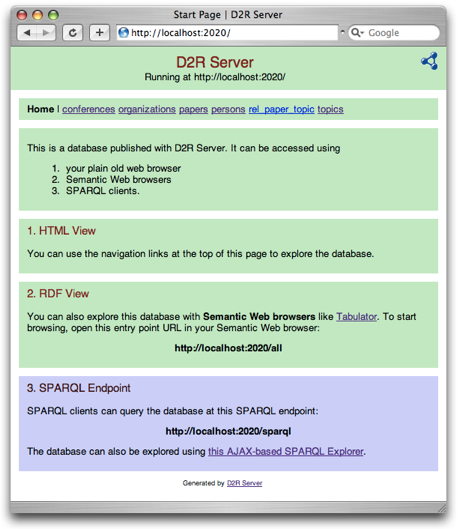
\includegraphics[scale=0.45]{d2r_server.png}\\
        \textbf{An example of a coin in the database}\footnotemark[6]%
        \label{fig:coin_example}%
    \end{minipage}%
    \begin{minipage}{0.5\textwidth}%
   With the d2r-server running locally, we are now able to view our data via either HTML or using a semantiv web browser. More importantly we are able to generate RDF dumps via the command line.
    \end{minipage}%
\end{figure}%

\begin{lstlisting}

# Generate a mapping file
generate-mapping -o mapping.ttl -d driver.class.name -u db-user -p db-password jdbc:url:...

# Start D2R Server
d2r-server mapping.ttl

# Generate an RDF dump
dump-rdf mapping.ttl -o dump.nt
\end{lstlisting}

\subsubsection{D2R Mapping Language}
The D2RQ mapping language is a declarative language used to map the data from the \textbf{D4N4} database to RDFS vocabularies. It is responsible for how the virtual RDF graph looks.\\
\underline{\textbf{Example}:}
\begin{center}
\begin{lstlisting}[language=Python]
map:coins a d2rq:ClassMap;
	d2rq:dataStorage map:database;
	d2rq:uriPattern "https://www.corpus-nummorum.eu/coins/@@data_coins.id@@";
	d2rq:class nmo:NumismaticObject;
	d2rq:condition "data_coins.publication_state = 1";
			.
\end{lstlisting}
\end{center}

In the example we are creating the 'd2rq:ClassMap' \textit{coins}, which represents one or multiple classes in the D2RQ Mapping Language. Instances of the class are being handled in accord to the definition in 'd2rq:ClassMap' by the D2RQ Mapping Language. In the next line reference to where the data is stored is given by mapping the database to 'd2rq:dataStorage'. In this case database is a variable defined earlier which represents a connection to the database. After this a reference to the resource is given by passing an URI pattern and an RDFS Class is being created. Every instance created from the ClassMap will also be an instance of this class. Lastly we are limiting the mapped coins to those with the value set accordingly, it functions as a SQL WHERE statement.
\subsubsection{D2R Server}
Ihr Text sollte unter Einbindung von Grafiken und Tabellen in Absätze gegliedert werden. Dabei ist zu beachten, dass ein Absatz einen thematischen Gedanken erfasst, wobei am Anfang des Absatzes im Regelfall die Kernaussage zu finden ist und von dieser ausgehend durch weitere Erörterungen innerhalb des Absatzes gegliedert wird

\newpage

\section{Assignment}
\subsection{Overview}
\subsection{Current state of the pipeline}
At the current state the steps of executing the pipeline are associated with a lot of manual work, starting from the manual execution of the NLP notebooks to the running from the D2RQ application. At the beginning of the pipeline the \textbf{NER} is being executed. The results of the \textbf{NER} builds the foundation on that the \textbf{RE} is build. In the notebook \textbf{NER} is being applied to every design of the database and the results are then uploaded again to the database. Afterwards, \textbf{RE} follows. As previously mentioned, \textbf{RE} takes as input a design, a subject and a object and tries to create a relationship between the subject and the object. With completion of the \textbf{RE} the created triples are uploaded to the database. The last step of the pipeline is the one, which requires the most amount of manual work and thereby offers the most room of improvement. In order to created the \textbf{RDF} data, the program \textbf{D2RQ}-server is launched. As mentioned, \textbf{D2RQ}-server builts the connection between the database and the \textbf{D2RQ} program. It allows us to apply a mapping, which will map the contents of our database to \textbf{RDF}. Lastly the execution of the mapping programm has to be done manually via the command line and the results is our data represented in RDF.
Summarized the pipeline looks like this:\\
\begin{center}
   \begin{tikzpicture}[auto,node distance=2cm,thick,main node/.style={circle,fill=blue!20,draw,font=\sffamily\Large\bfseries}, scale=2]
    \node[main node, rectangle, label=Test1,minimum size=1.5cm] (A) at (0,0) {Description};
    \node[main node, rectangle, label=Test2,minimum size=1.5cm ] (B) at (0,-2) {Output};
    \node[main node, rectangle, label=Test3,minimum size=1.5cm ] (C) at (0,-4) {Triples};
    \path [->] (A) edge node {\textbf{NER}} (B);
    \path [->] (B) edge node {\textbf{RE}} (C);
    
    \end{tikzpicture}
\end{center}

\subsection{Implementation of the revised pipeline}

\section{Results}
\subsection{Results}
\subsection{Comparison to the previous pipeline}
\newpage
\section{Conclusion and outlook}
\newpage
\section{List of figures}
\newpage
\section{Literature}
\printbibliography




\end{document}